\scanpage{4}
\mspage{2}
\figure{
\begin{tikzpicture}[x=.009cm,y=-.009cm,font=\small]
% The cancelled passage has three separate enclosing strokes, not a closed box.
\node[anchor=west,inner sep=0pt] at (240,125) {\deleted{s'envoie injectivement dans un groupe algébrique}};
\node[anchor=west,inner sep=0pt] at (240,215) {\deleted{commutatif de rang unipotent nul}};
\node[anchor=west,inner sep=0pt] at (250,305) {\deleted{(i.e. ext. d'une VA par un tore) alors}};
\node[anchor=west,inner sep=0pt] at (260,412) {\deleted{\uline{l'application}}};
\node[anchor=west,inner sep=0pt] at (570,480) {\begin{tikzcd}[ampersand replacement=\&,column sep=18mm]
{\deleted{X(\overline{\mathbf Q})}}\arrow[r]\&{\deleted{J}}
\end{tikzcd}};
\draw[line width=.4pt] (230,130)..controls(650,100)and(1190,99)..(1580,125);
\draw[line width=.4pt] (245,155)..controls(235,230)and(223,350)..(224,392)
 ..controls(224,406)and(228,412)..(233,402);
\draw[line width=.4pt] (526,440)..controls(520,466)and(516,501)..(531,516)
 ..controls(590,536)and(730,507)..(945,513)
 ..controls(929,475)and(922,387)..(922,348)
 ..controls(1010,330)and(1365,347)..(1552,329);
% Oblique cancellation is retained as physical ink, not counted as another error.
\draw[line width=.35pt] (484,140)--(367,371) (837,126)--(572,488)
 (1094,142)--(814,468) (1436,148)--(1258,296) (1577,153)--(1514,284);
\end{tikzpicture}
}

\textcircled{3} Supposons $X$ de t.f. sur $\overline{\mathbf Q}$. Alors on a
un ``germe de relèvement'' de $\Gamma$
\diagram{$(9)\qquad$
\begin{tikzcd}[ampersand replacement=\&]
\mathcal G_{\overline X}\arrow[r]\&\Gamma\arrow[d,phantom,"\cup" description]\\
\&\Gamma'\arrow[ul]
\end{tikzcd}}

sur ss-groupe ouvert (modulo la relation
de coïncidence sur un ss groupe
ouvert plus petit). Pour 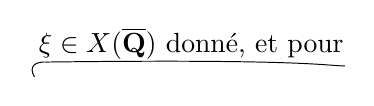
\begin{tikzpicture}[baseline=(base)]
\coordinate (base) at (0,-.23);
\node[anchor=south west,inner sep=0pt] (xinote) at (0,0) {\inserted{$\xi\in X(\overline{\mathbf Q})$ donné, et pour}};
\draw[line width=.35pt] ([xshift=-.05cm,yshift=-.22cm]xinote.south west)
 ..controls ([xshift=-.13cm,yshift=-.08cm]xinote.south west) and ([xshift=-.04cm,yshift=-.02cm]xinote.south west)..([xshift=.12cm,yshift=-.03cm]xinote.south west)
 ..controls ([xshift=-.50cm,yshift=.01cm]xinote.south east) and ([xshift=-.20cm,yshift=-.08cm]xinote.south east)..([xshift=.01cm,yshift=-.08cm]xinote.south east);
% Only the definite sweep is copied; its far-right extent merges with crease/edge.
\end{tikzpicture}
$\Gamma'$ assez petit,
\inserted{de $\xi$} $\Gamma'
\mathrel{\vcenter{\hbox{\begin{tikzpicture}[x=1mm,y=1mm]
\draw[line width=.45pt] (0,0)--(6,0)--(6,-.4);
\end{tikzpicture}}}}
\mathcal G_{\overline X}$ se factorise par $\mathcal G_{\overline X}(\xi)$, de
\margin{$X=\overline X$}
sorte qu'on a un 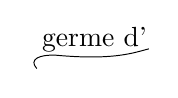
\begin{tikzpicture}[baseline=(base)]
\coordinate (base) at (0,-.22);
\node[anchor=south west,inner sep=0pt] (germe) at (0,0) {\inserted{germe d'}};
\draw[line width=.35pt] ([xshift=-.06cm,yshift=-.20cm]germe.south west)
 ..controls ([xshift=-.17cm,yshift=-.08cm]germe.south west) and ([xshift=-.02cm,yshift=-.02cm]germe.south west)..([xshift=.18cm,yshift=-.03cm]germe.south west)
 ..controls ([xshift=-.40cm,yshift=-.10cm]germe.south east) and ([xshift=-.15cm,yshift=.01cm]germe.south east)..([xshift=.02cm,yshift=.05cm]germe.south east);
\end{tikzpicture} hom composé
\[
\begin{gathered}
\hspace{1.6cm}\inserted{\Gamma'\mathrel{\vcenter{\hbox{\begin{tikzpicture}[x=1mm,y=1mm]
\draw[line width=.45pt,line cap=round] (0,0)..controls(2,.12)and(5,.48)..(6.6,.32);
\draw[line width=.45pt,line cap=round] (7,.8)--(7.3,.2)--(6.95,-.1);
\end{tikzpicture}}}}\mathcal E_X}\\[-.2em]
\deleted{\Gamma'\longrightarrow\mathcal E_X}\hspace{1.6cm}
\end{gathered}
\]
rendant commutatif
\diagram{$(10)\qquad$
\begin{tikzcd}[ampersand replacement=\&]
\mathcal E_X\arrow[r]\&\mathcal G_X\arrow[r]\&\Gamma\\
\&\&\Gamma'\arrow[u,hook]\arrow[ull,"{\varphi_\xi^t}"{below}]
\end{tikzcd}}

-- du moins si $\widetilde X=\widetilde X(\xi)$ -- sinon un
hom defini mod composition par un \unsure{autom}
int. provenant de $\pi_1(X)$. \unsure{Soulignons}
\mspage{3}
